
\section{Results}
\subsection{TSS applied to real-life networks}

We apply the TSS algorithm to real-life networks and compare it to the previously developed algorithm and a greedy version of TSS. The threshold of the nodes are set as $t(v)\in(1,2,...,10)$ for each iteration. For the random version of algorithms if more than one node meets the condition of cases we randomly selected a node from the set of nodes that satisfy the condition in each algorithm. The selection of nodes in case 3 of TSS can be randomized. We test if randomness of selection of nodes affect the cardinality of the target set and the runtime of the algorithm.

We get our data from real-life networks\cite{datasets1}\cite{datasets2}. The following datasets are used:
\begin{enumerate}
	\item BlogCatalog3 (10,312 nodes, 333,983 edges): a social blog directory which manages the bloggers and their blogs. Both the contact network and selected group membership information are included.
	\item Ca-AstroPh(18,772 nodes, 198,110 edges): Arxiv ASTRO-PH (Astro Physics) collaboration network is from the e-print arXiv and covers scientific collaborations between authors papers submitted to Astro Physics category.
	\item Ca-CondMat (23,133 nodes, 93,497 edges): Arxiv COND-MAT (Condense Matter Physics) collaboration network is from the e-print arXiv and covers scientific collaborations between authors papers submitted to Condense Matter category.
	\item Ca-GrQc (5,242 nodes, 14,496 edges): Arxiv GR-QC (General Relativity and Quantum Cosmology) collaboration network is from the e-print arXiv and covers scientific collaborations between authors papers submitted to General Relativity and Quantum Cosmology category. 
	\item Ca-HepPh (12,008 nodes, 118,521 edges): Arxiv HEP-PH (High Energy Physics - Phenomenology) collaboration network is from the e-print arXiv and covers scientific collaborations between authors papers submitted to High Energy Physics - Phenomenology category.
	\item Ca-HepTh (9,877 nodes, 25,998 edges): Arxiv HEP-TH (High Energy Physics - Theory) collaboration network is from the e-print arXiv and covers scientific collaborations between authors papers submitted to High Energy Physics - Theory category. 
\end{enumerate}

\begin{figure}
	\centering
	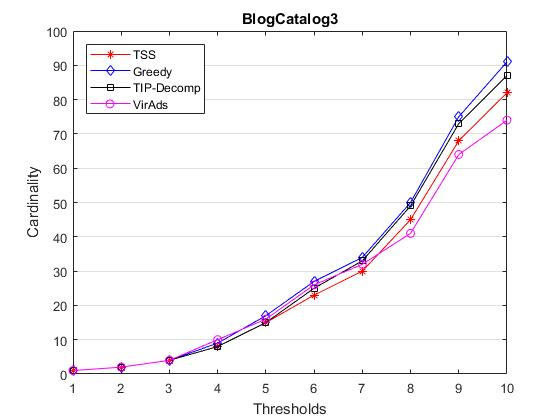
\includegraphics[scale=0.5]{images/bc3result.jpg}
	\caption{BlogCatalog3}
	\end{figure}
	
\begin{figure}
	\centering	
	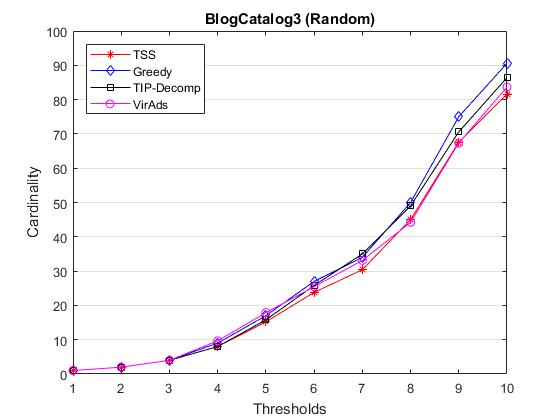
\includegraphics[scale=0.5]{images/bc3resultrandom.jpg}
	\caption{BlogCatalog3 Random}
	\end{figure}
\begin{figure}
	\centering	
	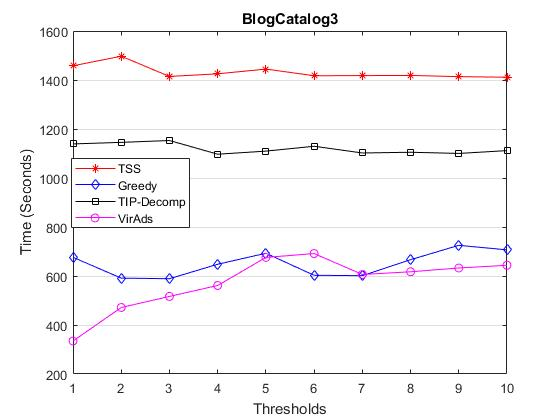
\includegraphics[scale=0.5]{images/bc3time.jpg}
	\caption{Runtime for BlogCatalog3 (seconds)}
\end{figure}

\begin{figure}
	\centering
	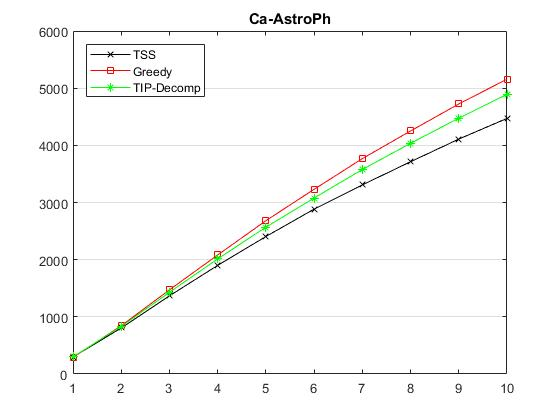
\includegraphics[scale=0.5]{images/ca-astrophresult.jpg}
	\caption{Ca-AstroPh}
	\end{figure}
\begin{figure}
	\centering	
	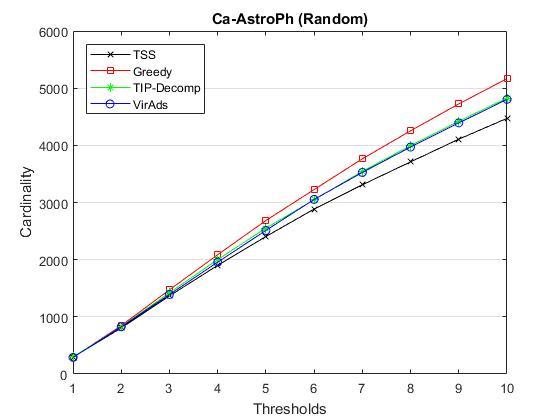
\includegraphics[scale=0.5]{images/ca-astrophresultrandom.jpg}
	\caption{Ca-AstroPh Random}
	\end{figure}
\begin{figure}
	\centering	
	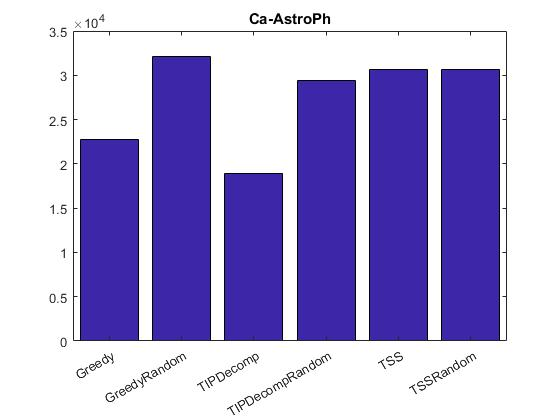
\includegraphics[scale=0.5]{images/astrophtime.jpg}
	\caption{Runtime for Ca-AstroPh (seconds)}
\end{figure}

\begin{figure}
	\centering
	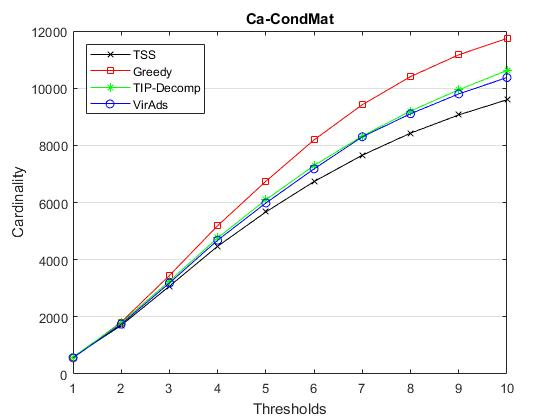
\includegraphics[scale=0.5]{images/ca-condmatresult.jpg}
	\caption{Ca-CondMat}
	\end{figure}
\begin{figure}
	\centering	
	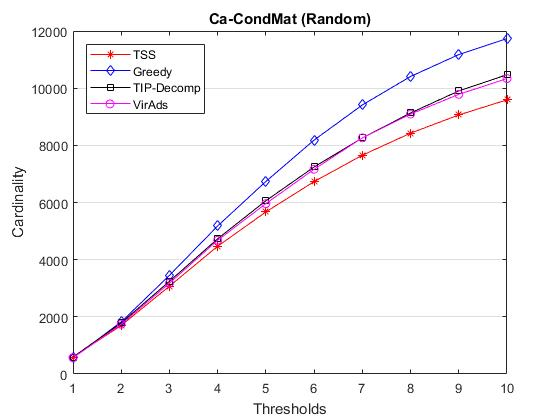
\includegraphics[scale=0.5]{images/ca-condmatresultrandom.jpg}
	\caption{Ca-CondMat Random}
	\end{figure}
\begin{figure}
	\centering	
	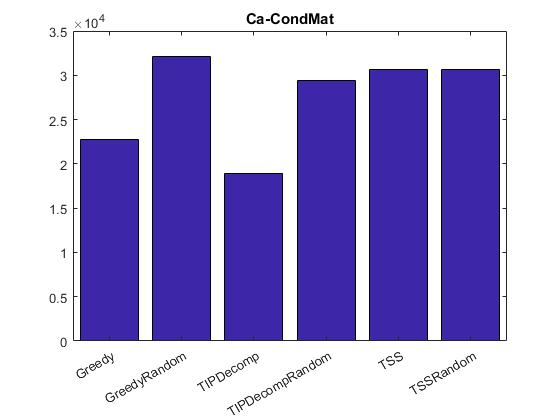
\includegraphics[scale=0.5]{images/condmathtime.jpg}
	\caption{Runtime for Ca-CondMat (seconds)}
\end{figure}

\begin{figure}
	\centering
	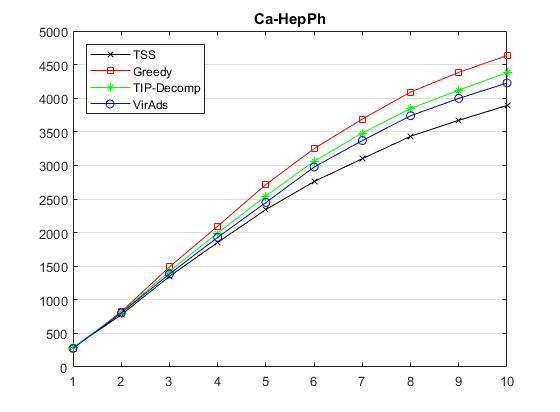
\includegraphics[scale=0.5]{images/ca-hepphresult.jpg}
	\caption{Ca-HepPh}
\end{figure}
\begin{figure}
\centering
	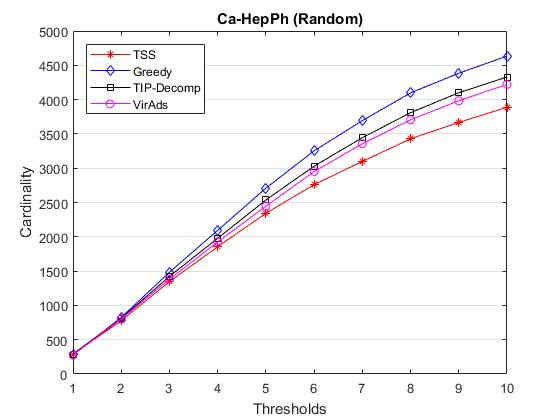
\includegraphics[scale=0.5]{images/ca-hepphresultrandom.jpg}
	\caption{Ca-HepPh Random}
	\end{figure}
\begin{figure}
	\centering	
	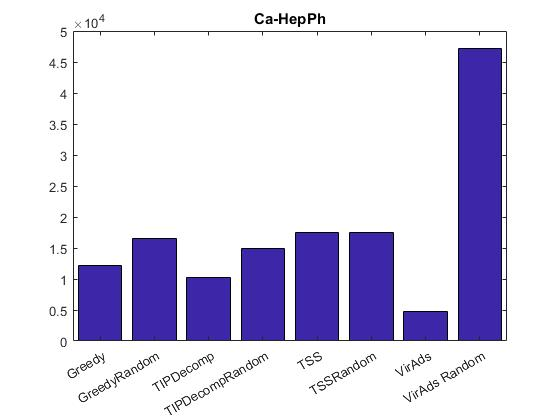
\includegraphics[scale=0.5]{images/hepphtime.jpg}
	\caption{Runtime for Ca-HepPh (seconds)}
\end{figure}

\begin{figure}
	\centering
	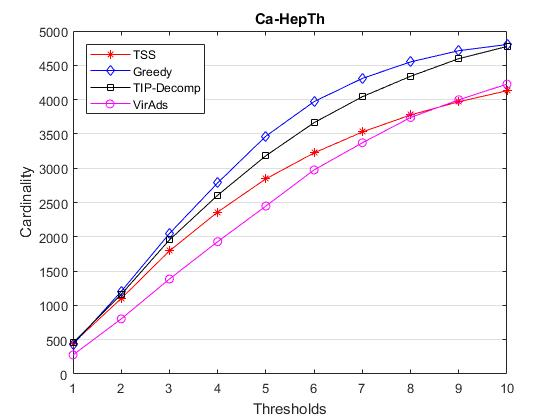
\includegraphics[scale=0.5]{images/ca-hepthresult.jpg}
	\caption{Ca-HepTh}
\end{figure}
\begin{figure}
	\centering	
	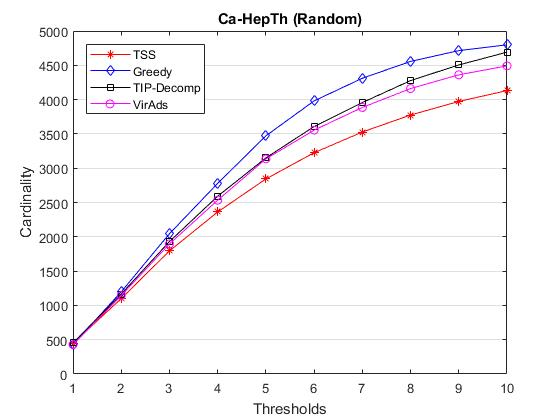
\includegraphics[scale=0.5]{images/ca-hepthresultrandom.jpg}
	\caption{Ca-HepTh Random}
\end{figure}
\begin{figure}
	\centering
	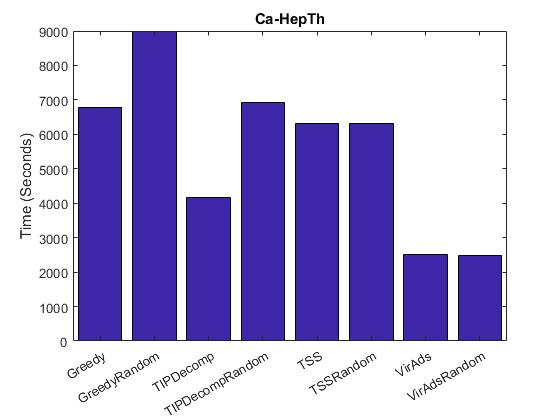
\includegraphics[scale=0.5]{images/hepthtime.jpg}
	\caption{Runtime for Ca-Hepth (seconds)}
\end{figure}
	
	
